\documentclass[11pt]{article}
\usepackage{coling2016}
\usepackage{times}
\usepackage{url}
\usepackage{latexsym}
\usepackage{graphicx}
\usepackage{amsmath}
\usepackage{scrextend}
\makeatletter
\renewcommand*{\p@section}{\S\,}
\renewcommand*{\p@subsection}{\S\,}
\makeatother


%\setlength\titlebox{5cm}
% You can expand the titlebox if you need extra space
% to show all the authors. Please do not make the titlebox
% smaller than 5cm (the original size); we will check this
% in the camera-ready version and ask you to change it back.

\newcommand\BibTeX{B{\sc ib}\TeX}

\title{Syntactic realization with data-driven neural tree grammars}

\author{Brian McMahan \and Matthew Stone \\
   Computer Science, Rutgers University \\
   {\tt brian.mcmahan, matthew.stone@rutgers.edu}}

\date{}

\begin{document}
\maketitle

%\vspace*{-0.5cm}
\begin{abstract}

A key component in surface realization in natural language generation
is to choose concrete syntactic relationships to express a target
meaning.
%
We develop a new method for syntactic choice based on learning a
stochastic tree grammar in a neural architecture.
%
This framework can exploit state-of-the-art methods for modeling word
sequences and generalizing across vocabulary.
%
We also induce embeddings to generalize over elementary tree
structures and exploit a tree recurrence over the input structure to
model long-distance influences between NLG choices.
%
We evaluate the models on the task of linearizing unannotated
dependency trees, documenting the contribution of our modeling
techniques to improvements in both accuracy and run time.

\end{abstract}

\section{Introduction}
%\vspace*{-0.2cm}


\blfootnote{
    % % final paper: en-us version (to licence, a license)
    %
    \hspace{-0.65cm}  % space normally used by the marker
    This work is licensed under a Creative Commons 
    Attribution 4.0 International License.
    License details:
    \url{http://creativecommons.org/licenses/by/4.0/}
}

Where natural language understanding systems face problems of
ambiguity, natural language generation (NLG) systems face problems of
choice. A wide coverage NLG system must be able to formulate messages
using specialized linguistic elements in the exceptional circumstances
where they are appropriate; however, it can only achieve fluency by
expressing frequent meanings in routine ways. Empirical methods have
thus long been recognized as crucial to NLG; see
e.g. \newcite{langkilde1998generation}.

With traditional stochastic modeling techniques, NLG researchers have
had to predict choices using factored models with handcrafted
representations and strong independence assumptions, in order to avoid
combinatorial explosions and address the sparsity of training data.
%
By contrast, in this paper, we leverage recent advances in deep
learning to develop new models for syntactic choice that free
engineers from many of these decisions, but still generalize more
effectively, match human choices more closely, and enable more
efficient computations than traditional techniques.

We adopt the characterization of syntactic choice from
\newcite{bangalore2000exploiting}: the problem is to use a stochastic
tree model and a language model to produce a linearized string from an
unordered, unlabeled dependency graph.
%
The first step to producing a linearized string is to assign each item
an appropriate \emph{supertag}---a fragment of a parse tree with a
leaf left open for the lexical item.
%
This process involves applying a learned model to make predictions for
the syntax of each item and then searching over the predictions to
find a consistent assignment for the entire sentence.
%
The resulting assignments allow for many possible surface realization
outputs because they can underdetermine the order and attachment of
adjuncts.
%
To finish the linearization, a language model is used to select the
most likely surface form from among the alternatives.
%
While improving the language model would improve the linearized string,
we focus here on more accurately predicting the correct supertags from
unlabeled dependency trees.

Our work exploits deep learning to improve the model of supertag
assignment in two ways.
%
First, we analyze the use of embedding techniques to generalize across
supertags.  
%
Neural networks offer a number of architectures that can cluster tree
fragments during training; such models learn to treat related structures
similarly, and we show that they improve supertag assignments.
%
Second, we analyze the use of tree recurrences to track hierarchical
relationships within the generation process.
%
Such networks can track more of the generation context than a simple
feed-forward model; as a side effect, they can simplify the problem of
computing consistent supertag assignments for an entire sentence.
%
We evaluate our contributions in two ways: first, by varying the
technique used to embed supertags, and then by comparing a
feed-forward model against our recurrent tree model.

Our presentation begins in \ref{sec:tree} with an introduction to tree
grammars and a deterministic methodology for inducing the elementary
trees of the grammar.
%
Next, \ref{sec:neural} presents the techniques we have developed to
represent a tree grammar using a neural architecture.
%
Then, in \ref{sec:models}, we describe the specific models we have
implemented and the algorithms used to exploit the models in NLG.
%
The experiments in \ref{sec:expt} demonstrate the improvement of the
model over baseline results based on previous work on stochastic
surface realization.
%
We conclude with a brief discussion of the future potential for neural
architectures to predict NLG choices.

\section{Tree Grammars}
\label{sec:tree}
%\vspace*{-0.2cm}

Broadly, tree grammars are a family of tree rewriting formalisms that
produce strings as a side effect of composing primitive
hierarchical structures.  The basic syntactic units are called
elementary trees; elementary trees combine using tree-rewrite rules to
form derived phrase structure trees describing complex sentences.
Inducing a tree grammar involves fixing a formal inventory of
structures and operations for elementary trees and then inferring
instances of those structures to match corpus data.

\subsection{Grammar Formalism}
%\vspace*{-0.1cm}

The canonical tree grammar is perhaps lexicalized tree-adjoining
grammar (LTAG) \cite{joshi1991tree}.
%
The elementary trees of LTAG consist of two disjoint sets with
distinct operations: initial trees can perform substitution operations
and auxiliary trees can perform adjunction operations.
%
The substitution operation replaces a non-terminal leaf of a target
tree with an identically-labeled root node of an initial tree.
%
The adjunction operation modifies the internal structure of a target
tree by expanding a node identically-labeled with the root and a
distinguished foot note in the auxiliary tree.
%
The lexicalization of the the grammar requires each elementary tree to
have at least one lexical item as a leaf.

LTAG incurs computational costs because it is mildly context-sensitive
in generative power.
%
Several variants reduce the complexity of the formalism by limiting
the range of adjunction operations.
%
For example, the Tree Insertion Grammar allows for adjunction as long as it is either a left or right auxiliary tree \cite{Schabes1995}.
%
Tree Substitution Grammars, meanwhile, allow for no adjunction and
only substitutions \cite{cohn2009inducing}.
%
We adopt one particular restriction on adjunction, called
sister-adjunction or \emph{insertion}, which allows trees to attach to
an interior node and add itself as a first or last child
\cite{chiang2000statistical}.
%
Chiang's sister-adjunction allows for the flat structures in
the Penn Treebank while limiting the formalism to context-free power.

\subsection{Grammar Induction}
%\vspace*{-0.1cm}

In lexicalized tree grammars, the lexicon and the grammatical rules
are one and the same.
%
The set of possible grammatical moves which can be made are simultaneously the set of possible words which can be used next.
%
This means inducing a tree grammar from a data set is a matter of inferring the set of constructions in the data.

%%%%\tabularnewline

We follow previous work in using bracketed phrase structure corpora
and deterministic rules to induce the grammar
\cite{bangalore2001impact,chiang2000statistical}.
%
Broadly, the methodology is to split the observed trees into the
constituents which make it up, according to the grammar formalism.
%
We use head rules
\cite{chiang2000statistical,collins1997three,magerman1995statistical}
to associate internal nodes in a bracketed tree with the lexical item
that owns it.
%
We use additional rules to classify some children as complements,
corresponding to substitution sites and root notes of complement
trees; and other children as adjuncts, corresponding to insertion
trees that combine with the parent node, either to the right or to the
left of the head.  This allows us to segment the tree into units of
substitution and insertion.%
\footnote{One particular downside of deterministically constructing
  the grammar this way is that it can produce an excess of superfluous
  elementary trees.
%
We minimize this by collapsing repeated projections in the treebank.
%
Other work has provided Bayesian models for reducing grammar
complexity by forcing it to follow Dirichlet or Pitman-Yor processes
\cite{Cohn2010}---an interesting direction for future work.}



\begin{figure*}[tH!]
\centering
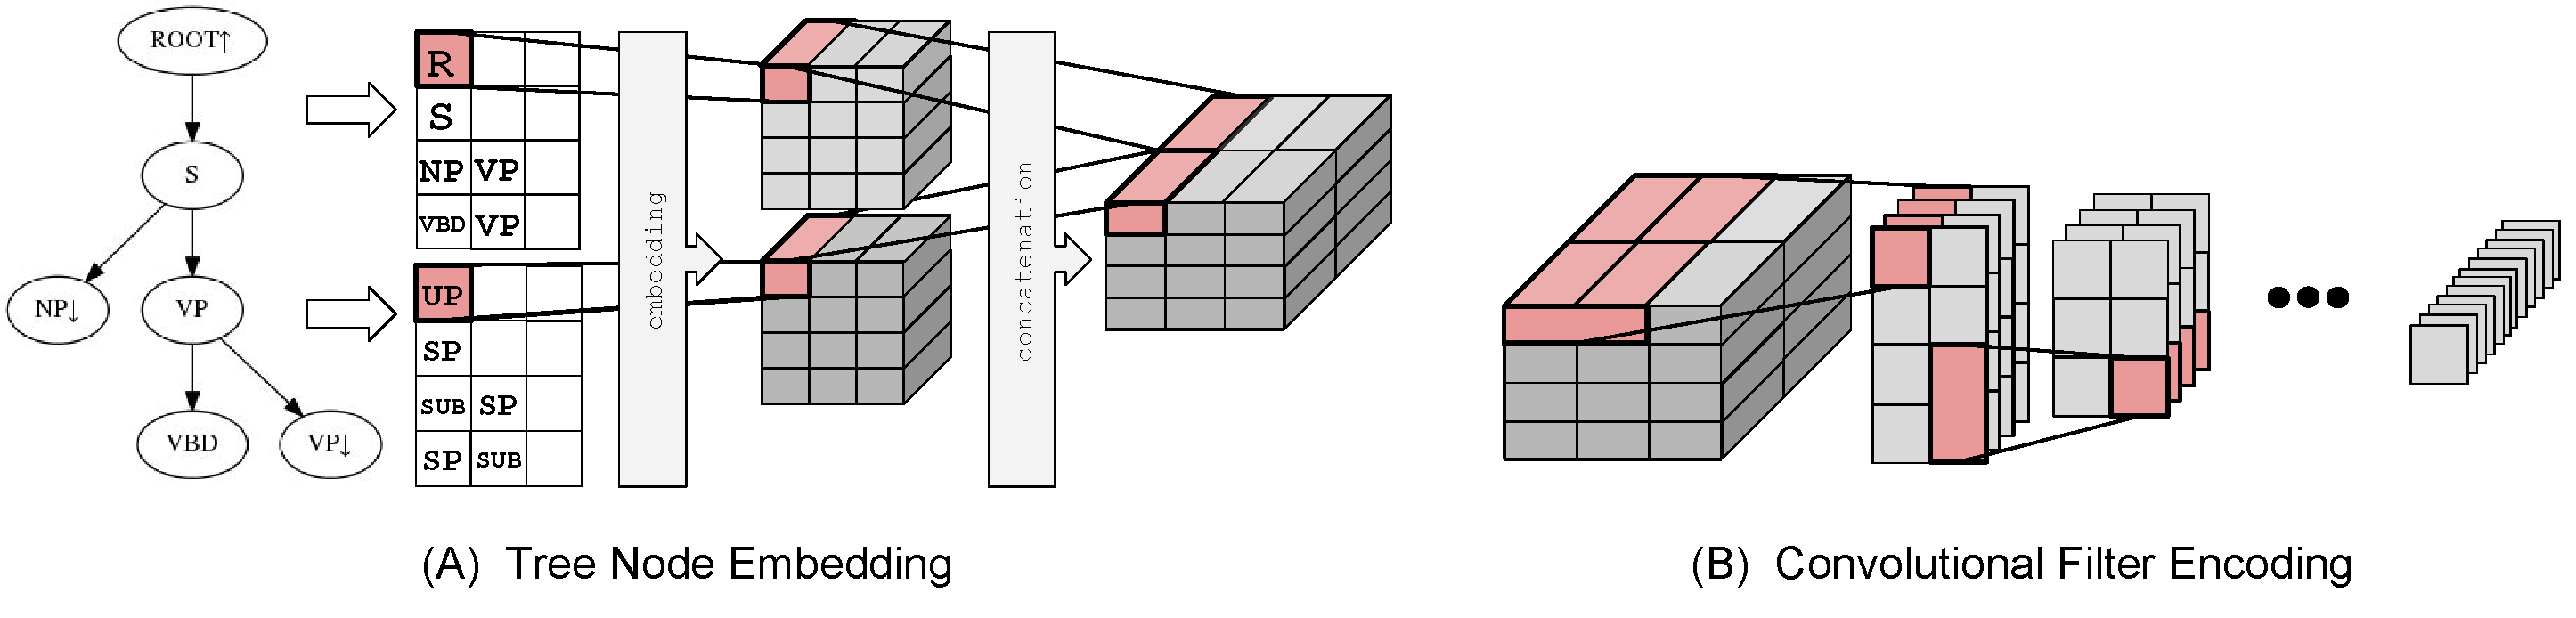
\includegraphics[width=\textwidth]{spineembed.pdf}
\caption{Embedding supertags using convolutional neural networks. In (A), a tree is encoded by its features and then embedded.
 In (B), convolutional layers are used to encode the supertag into a vector.}
 \label{fig:spineembedding}
%\vspace*{-0.5cm}
\end{figure*}



\section{Neural Representations}
\label{sec:neural}
%\vspace*{-0.2cm}

The grammar induction of \ref{sec:tree} allows us to construct an
inventory of supertags to match a corpus.  For NLG, we also need to
predict the most likely supertag for any lexical item given the
generation context.  We approach this problem using neural
networks. 
%
In particular, this work makes two contributions to improve stochastic
tree modeling with neural networks.
%
First, we represent supertags as vectors through embedding techniques
that enable to model to generalize over complex, but related
structures.
%
Second, we address the hierarchical dependence between choices using a
recurrent tree network that can capture long-distance influences as
well as local ones.
%
We now describe these representations in more detail.

\subsection{Embedding Supertags}
%\vspace{-0.1cm}

Different supertags for the same word can encode differences in the
item's own combinatorial syntax, differences in argument structure, and
differences in word order.  Accordingly, words have many related
supertags, with substantial overlaps in structure, and, presumably,
corresponding similarities in their patterns of occurrence.  A
traditional machine learning approach to supertag prediction would
treat individual supertags as atoms for classification; generalizing
across supertags would require linking model parameters to handcrafted
features or back-off categories.

By contrast, neural techniques work by embedding such tokens into a
vector space. This process learns an abstract representation of tokens
that clusters similar items together and makes further predictions
as a function of those items' learned features.  The resulting
ability to generalize across sparse data seems to be one of the most
important reasons for the success of deep learning in NLP.

The simplest way to embed supertags is to treat each structure
as a distinct token that indexes a corresponding learned vector.  This
places no constraints on the learned similarity function, but it also
ignores the hierarchical structure of the elementary trees
themselves.  Previous work on deep learning with graph structures
suggests convolutional neural networks can exploit similarities in structure \cite{niepert2016learning,kalchbrenner2014convolutional}.  Thus, we developed
analogous techniques to encode supertags based on their underlying
tree structure.  In particular, to embed a supertag, we embed each
node, group the resulting vectors to form a tensor, and then summarize
the tensor into a single vector using a series of convolutional neural
networks.

Note that each elementary tree is a complex structure with nodes
labeled by category and assigned a role that enables further tree
operations.
%
The root node's role represents the overall action associated with
that elementary tree---either substitution or insertion.
%
The remaining nodes either have the substitution point role or the
spine role---they are along the spine from root to the lexical
attachment point, and thus provide targets for further insertion.

We first embed each node independently, then combined the vectors to
form a tensor of embeddings.
%
Specifically, symbols representing the syntactic category and node
roles are treated as distinct vocabulary tokens, mapped to integers,
and used to retrieve a vector representation that is learned during
training.
%
The vectors are grouped into a tensor by placing the root node into
the first cell of the first row and left-aligning the descendants in
the subsequent rows.
%
The two tensors are concatenated along the embedding dimension.
%
This embed-and-group method is shown in on the left in Figure \ref{fig:spineembedding}.
%the root node is in first cell in the first row and the subsequent nodes are


Using a series of convolutional neural networks which learn their weights during training, the tensor of embeddings can be reduced to a single vector.
%
To reduce the tensor to a vector, the convolutions are designed with increasingly larger filter sizes.
%The convolutions are applied with increasingly larger filter sizes, leading to a reduction in dimensions.
%
Additionally, the dimensions are reduced alternatingly to also facilitate the capture of features.
%
The entire process is summarized in Eq. \ref{eq:embed} with $\Lambda$ representing the supertags, $G$ representing embedding matrices, and
$C$ representing the convolutional neural network layers.
%
Specifically, $G_s$ is the syntactic category embedding matrix and
$G_r$ is the node role embedding matrix.
%
Each convolutional layer $C$ is shown with its corresponding height and width as $C^{i,j}$.
%
The encoding first constructs the tensor, $T_\Lambda$, through the embed-and-group method.
%
Then, the embedding matrix $G_\Lambda$ is summarized from $T_\Lambda$ using the
series of convolutional layers.
%
%\vspace*{-0.5cm}
\begin{align}
& T_\Lambda = [G_s(\Lambda_{syntactic~category});~G_r(\Lambda_{role})] \nonumber \\
& G_\Lambda = C^{4,5}(C^{3,1}(C^{1,3}(C^{2,1}(C^{1,2}(T_\Lambda))))) \label{eq:embed}
\end{align}
%\vspace*{-0.5cm}
%
The final product, a vector per supertag, is aggregated with the other vectors
and turned into an embedding matrix.
%
This is visualized in on the right in Figure \ref{fig:spineembedding}.
%
During training and test time, supertags are simply input as indices
and their feature representations retrieved as an embedding.


%%%%
\subsection{Recurrent Tree Networks}
\label{subsec:rtn}
%\vspace{-0.1cm}

\begin{figure*}[tH!]
\centering
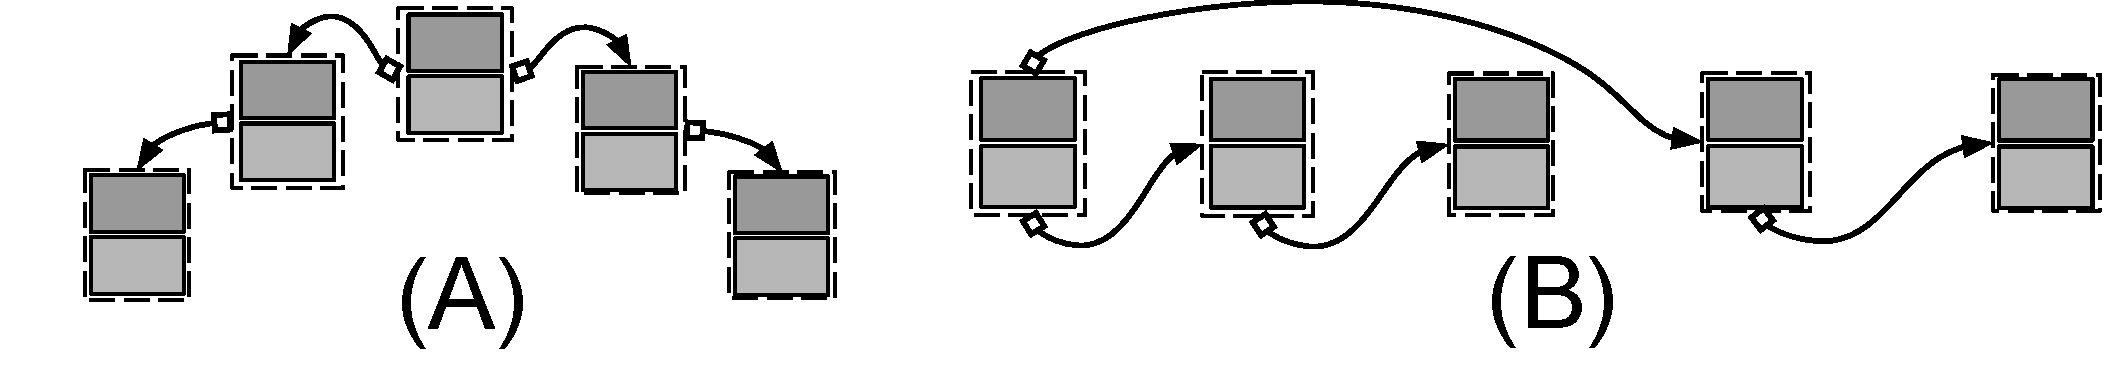
\includegraphics[width=0.8\textwidth]{rtn2.pdf}
\caption{A recurrent tree network. (A) The dependency structure as a tree.  (B) The dependency structure as a sequence.}
 \label{fig:rtn}
%\vspace*{-0.5cm}
\end{figure*}

Our models predict supertags as a function of the target word and its
context.  Neural networks make it possible to generalize over such
contexts by learning to represent them with a hidden state vector that
aggregates and clusters information from the relevant history.  Our
approach is to do this using a recurrent tree network.
%
While recurrent neural networks normally use the previous hidden state in the sequential order of the inputs,
%require  the hidden state to be from the
%temporally previous hidden state,
recurrent tree networks use the hidden state from the parent.
%
Utilizing the parent's hidden state rather than the sequentially previous hidden
state, the recurrent connection can travel down the branches of a tree.
%
An example of a recurrent tree network is shown in Figure \ref{fig:rtn}.



In our recurrent tree network, child nodes gain access to a parent's hidden state
through an internal \emph{tree state}.
%
During a tree recurrence, the nodes in the dependency graph are enumerated in a
top-down traversal.
%
At each step in the recurrence, the resulting recurrent state is stored in the
tree state at the step index.
%
Descendents access the recurrent state using a topological index that is passed in as data.

The formulation is summarized in Equation \ref{eq:rnnsetup}.
%
The input to each time step in the current tree is the data, $x_t$, and a topological
index, $p_t$.
%
The recurrent tree uses $p_t$ to retrieve the parent's hidden state, $s_p$, from the
tree state, $S_{tree}$, and applies the recurrence function, $g(\dot)$.
%
The resulting recurrent state is the hidden state for child node, $s_c$.
%
The recurrent state $s_c$ is stored in the tree state, $S_{tree}$, at index $t$.
%
%\vspace*{-0.5cm}
\begin{align}
       s_c~&=~RTN(x_t,p_t) \nonumber \\
           &=~g(x_t,S_{tree}[p_t]) \nonumber \\
           &=~g(x_t, s_p) \nonumber \\
S_{tree}[t]&=~s_c \label{eq:rnnsetup}
\end{align}
%\vspace*{-0.5cm}
%
The use of topological indices allows for many recurrent tree networks to be
run in parallel on a GPU for efficiency.
%
GPU implementations must be formulated homogeneously so that 
the same operations are applied across the entire data structure.
%
Normally, tree operations involve conditional access to parent nodes,
but using topological indices and a tree state accesses the parent in
a homogeneous way.

\section{Models}
\label{sec:models}
%\vspace*{-0.2cm}

To analyze the representations we describe in \ref{sec:tree} and
\ref{sec:neural}, we developed two alternative architectures for
predicting supertags in context.
%
The first is a feed-forward neural network designed to solve a closely
analogous task to the supertagging step of
\newcite{bangalore2000exploiting}'s original FERGUS model.
%
We call it Fergus-N (for Neuralized).
%
The second uses a recurrent tree network to model the generation
context.
%
Because it has this richer context representation, it takes advantage
of a slightly different characterization of the supertag prediction
problem to streamline the problem solving involved in using the model.
%
We call this Fergus-R (for Recurrent).

For both stochastic tree models, a recurrent neural network language model is used to complete the linearization task.
%Both models produce partial results which a recurrent neural network language model is used to complete the linearization task.
%
%It is important to note that it is the same language model
%By using the same language model to finishing linearizing the output of both models, any observed differences in performance can be localized to the performance of the stochastic tree models.
%
The same language model is used to eliminate the confound of
language model performance and measure performance differences in the
stochastic tree modeling.
%

\subsection{Model 1: Fergus-N}
%\vspace{-0.1cm}

Fergus-N is a stochastic tree model which uses local parent-child information as inputs to a feed-forward network.
%
Each parent-child pair is treated as independent of all others.
%
The probability of the parent's supertag is predicted using an embedding of the pair's lexical material and an embedding of the child's supertag.
%
(Our experiments compare the different embedding options surveyed in
\ref{sec:neural}.) 
%
Training maximizes the likelihood of the training data according to
the model.
%
Formally, our objective is to minimize the negative log probability of
the observed parent supertags for each parent-child pair, as formally
defined in Eq. \ref{eq:fergusn_obj}.
%
%\vspace*{-0.55cm}
\begin{align}
&min_{\theta} -[\sum_p\sum_{p\to c} log[P_\theta(tag_{p} | lex_{p}, lex_{c}, tag_{c})] + \sum_c log[P_\theta(tag_{c} |lex_{p}, lex_{c})]] \label{eq:fergusn_obj}
\end{align}
%\vspace*{-0.45cm}
%
Here $tag_p$ is the parent
supertag, $tag_c$ is the child supertag, $lex_p$ is the parent's
lexical material, and $lex_c$ is the child's lexical material.
%
Note that the probability of supertags for the leaves of the tree are computed
with respect to their parent's lexical material.

The model is implemented as a feed-forward neural network.
%
Equation \ref{eq:fergusn} details the model formulation.
%
The lexical material, $lex_p$ and $lex_c$, are embedded using the word embedding matrix, $G_w$, concatenated, and mapped to a new vector, $\omega_{lex}$, with a fully connected layer, $FC_1$.
%
The child supertag, $tag_c$, is embedded with $G_\Lambda$ and concatenated the lexical vector, $\omega_{lex}$, forming an intermediate vector representation of the node, $\omega_{node}$.
%
The node vector is repeated for each of the parent's possible supertags, $tagset_p$, and then concatenated with their embeddings to construct the set of treelet vectors, $\Omega_{treelet}$.
%
The vector states for the leaf nodes are similarly constructed, but instead combine the lexical vector, $\omega_{lex}$ with the embeddings of the child's possible supertags, $tagset_c$.
%
The final operation induces a probability distribution over the treelet and leaf vectors using a score computed by the vectorized function, $\Psi_{predict}$, as the scalar in a softmax distribution. 
%
%\vspace*{-0.55cm}
\begin{align}
&\omega_{lex} = FC_1([G_w(lex_p); G_w(lex_c)]) \label{eq:fergusn} \\
&\omega_{node}=concat([G_\Lambda(tag_c);~\omega_{lex}]) \nonumber \\
&\Omega_{treelet} = concat([repeat(\omega_{node}),~G_\Lambda(tagset_p)]) \nonumber \\
&\Omega_{leaf} = concat([repeat(\omega_{lex}),~G_\Lambda(tagset_c)]) \nonumber \\
&P_\theta(tag_{p,i} | lex_{p}, lex_{c}, tag_{c})=
\frac{exp(\Psi_{predict}(\omega_{treelet_i})))}
{\sum_{j \in |tagset_p|} exp(\Psi_{predict}(\omega_{treelet_j})))} \nonumber \\
&P_\theta(tag_{c,i} |lex_{p}, lex_{c}) = 
\frac{exp(\Psi_{predict}(\omega_{leaf_i})))}
{\sum_{j \in |tagset_c|} exp(\Psi_{predict}(\omega_{leaf_j})))} \nonumber 
\end{align}
%\vspace*{-0.45cm}

At generation time, we are given a full dependency tree.  A decoding
step is necessary to compute a high probability assignment for all
supertags simultaneously.
%
In this process, tags for children must be chosen consistently with
one another, and the resulting probabilistic information must be
propagated upward to rerank tags higher in the tree.
%
We solve this problem with an A* algorithm.
%
At each step, the algorithm uses a priority queue to select subtrees based on their inside-outside scores.
%
The inside score is computed as the sum of the log probabilities of the supertags in the subtree.
%
The outside score is the sum of the best supertag for nodes outside the subtree, similar to \newcite{lewis2014improved}.
%
Once selected, the subtree is attached to the possible supertags of its parent that are both locally consistent and consistent among its already attached children.
%
These resulting subtrees are placed into the priority queue and the algorithm iterates to progress the search.
%
The search succeeds when the first complete tree has been found.\footnote{Although, the data has some noise so that sometimes there is no complete tree that can possibly be formed.}

\subsection{Model 2: Fergus-R}
%\vspace{-0.1cm}

Fergus-R is a stochastic tree model implemented in a top-down recurrent tree network and augmented with soft attention.
%
For each node in the input dependency tree, soft attention---a method which learns a vectorized function to weight a group of vectors and sum into a single vector---is used to summarize its children.
%
The soft attention vector and the node's embedded lexical material serve as the input to the recurrent tree.
%
The output of the recurrent tree represents the vectorized state of each node and is combined with each node's possible supertags to form prediction states.
%
%The recurrent tree output and the embedded supertag of the node's parent are used to compute a probability distribution over supertags.
%
%Using only summarized lexical information from its ancestors and children, the model computes a probability distribution over supertags for each node's recurrent tree output.
%
%so that the soft attention and recurrence relationships are only communicating lexical information.
Importantly, removing the conditional dependence on descendents' supertags
results in the simplified objective function in Eq. \ref{eq:rtnobj} where $lex_C$ is the children's lexical information, $lex_p$ is the parent's lexical information, $tag_p$ is the supertag for the parent node, and $RTN$ is the recurrent tree network. 
%
%\vspace*{-0.55cm}
\begin{align}
&min_{\theta} -[\sum_{(p,C)} P_\theta(tag_{p}|RTN,~lex_p,~lex_{C})] \label{eq:rtnobj}
\end{align}
%\vspace*{-0.45cm}

The Fergus-R model uses only lexical information as input to calculate the probability distribution over each node's supertags. 
%
The specific formulation is detailed in Eq. \ref{eq:fergusr}.
%
First, a parent node's children, $lex_C$, are embedded using the word embedding matrix, $G_w$, and then summarized with an attention function, $\Psi_{attn}$, to form the child context vector, $\omega_{C}$. 
%
The child context is concatenated with the embedded lexical information of the parent node, $lex_p$, and mapped to a new vector space with a fully connected layer, $FC_1$, to form the lexical context vector, $\omega_{lex}$.
%
The context vector and a topological vector for indexing the internal tree state (see \ref{subsec:rtn}) are passed to the recurrent tree network, $RTN$, to compute the full state vector for the parent node, $\omega_{node}$.
%
Similar to Fergus-N, the state vector is repeated and concatenated with the vectors of the parent node's possible supertags, ${tagset}_p$, and mapped to a new vector space with a fully connected layer, $FC_2$.
%
A vector in this vector space is labeled $\omega_{elementary}$ because the combination of supertag and lexical item constitutes an elementary tree.
%
The last step is to compute the probability of each supertag using the vectorized function, $\Psi_{predict}$.
%
%\vspace*{-0.55cm}
\begin{align}
&\omega_{C} = \Psi_{attn}(G_w(lex_C)) \label{eq:fergusr} \\
&\omega_{lex} = FC_1(concat(\omega_{C},~G_w(lex_p))) \nonumber \\
&\omega_{node} = RTN(\omega_{lex},~topology) \nonumber \\
&\Omega_{elementary} = FC_2(concat(repeat(\omega_{node}),~G_\Lambda(tagset_p))) \nonumber \\
&P_\theta(tag_{p,i}~|~RTN,~lex_p,~lex_{C}) = 
\frac{exp(\Psi_{predict}(\omega_{elementary_i})))}
{\sum_{j \in |\Omega|} exp(\Psi_{predict}(\omega_{elementary_j))}} \nonumber
\end{align}
%\vspace*{-0.45cm}

Although the same A* algorithm from Fergus-N is used, the decoding for Fergus-R is far simpler.
%
As supertags are incrementally selected in the algorithm, the inside score of the subsequent subtree is computed.  
%
Where Fergus-N had to compute a incremental dynamic program to evaluate the inside score, Fergus-R decomposes into a sum of conditionally independent distributions. 
%
The resulting setup is a chart parsing problem where the inside score of combining two consistent (non-conflicting) edges is just the sum of their inside scores. 

\subsection{Linearization}
%\vspace{-0.1cm}

The final step to linearizing the output of Fergus-N and Fergus-R---a dependency tree annotated with supertags and partial attachment information---is a search over possible orderings with a language model. 
%
There are many possible orderings due to adjunction operation
What remains to be determined is the order in which adjuncts are attached. 
%
Following \newcite{bangalore2000exploiting}, a language model is used to select between the alternate orderings. 
%
The language model used is a two-layer LSTM trained using the Keras library on
the surface form of the Penn Treebank.
%
The surface form was minimally cleaned\footnote{With respect to the surface form, the only
cleaning operations were to merge proper noun phrases into single tokens.  Punctuation and other
common cleaning operations were not performed.} to simulate realistic scenarios.

The difficulty of selecting orderings with a language model is that the possible linearizations can grow exponentially.
%
In particular, our implementations result in a large amount of insertion trees.\footnote{Many of the validation examples had more than $2^{40}$ possible linearizations.}
%
We approach this problem using a prefix tree which stores the possible linearizations as back-pointers to their last step and the word for the current step. 
%
The prefix tree is greedily searched with 32 beams.




\section{Experiments}
\label{sec:expt}
%\vspace*{-0.2cm}

Using the representations of \ref{sec:neural}, the models of
\ref{sec:models} can be instantiated in six different ways.  We can
use a feed-forward Fergus-N architecture or a recurrent Fergus-R
architecture.  Each architecture can embed supertags \emph{minimally},
by learning a scalar corresponding to each supertag; \emph{atomically}, by learning an
embedding vector corresponding to each supertag; or
\emph{structurally}, by using convolutional coding over each
supertag's tree structure to form a vector.
%
In each case, the vector (a size-one vector in the \emph{mimimal} condition) is concatenated as described in \ref{sec:models}.

\subsection{Training}
%\vspace{-0.1cm}

We trained six such models using a common experimental platform.  We
started from the Wall Street Journal sections of the Penn Treebank,
which have been previously used for evaluating statistical tree
grammars \cite{chiang2000statistical}.\footnote{A possible additional
  data source, the data from the 2011 Shared Task on Surface
  Realization, was not available.}
%
Our data pipeline breaks each sentence in the treebank into component
elementary trees and then represents the sentence in terms of a
derivation tree, specifying the tree-rewriting operations required to
construct the actual treebank surface tree from the basic supertags.
%
Removing supertags from the derivation tree leads to the unlabeled
dependency trees our models assume as input.

From this input, we extracted the atomic supertag prediction instances
and trained a network defined by each of the architectures of
\ref{sec:models} and each of the supertag representations of
\ref{sec:neural}.  As always, we used Section 02-21 for training,
Sections 22 for development, and Section 23 for testing.  A complete
description of network organization and training parameters is given
in the appendix.  The code and complete experimental setup are
publically
available.\footnote{\url{https://github.com/braingineer/neural_tree_grammar}}

\subsection{Performance Metrics}
%\vspace{-0.1cm}


We evaluate the performance of the models in several ways.  First, we
look at the accuracy of the supertag predictions directly output by
each model.  Second, we look at the accuracy of the final supertags
obtained by decoding the model predictions to the best-ranked
consistent global assignment.  These metrics directly assess the
ability of the models to successfully learn the target distributions.

Next, we evaluate the models on the full NLG task, including
linearization.  
%
The linearization task allows more freedom in supertag
classifications because supertags may differ in minor ways, such as
the projections present along the spine, which will not affect
generation output for a particular target input.
%
The freedom means models may not be penalized based on decisions that
don't matter---thus, at the same time, it also mutes the
distinctions between classification decisions.
%
We report a modified edit distance measure, Generation String Accuracy, following \cite{bangalore2000evaluation}.
%
%They argue that their measure correlates with NLG performance better
%than n-gram counting methods.
%
Since linearization uses a beam search, we report statistics both for
the top-ranked beam and for the empirically based beam among the
candidates computed during search.
%
The difference gives an indication of the effect of the language model
in guiding the decisions that remain after supertagging.

Finally, we report statistics about the run time of different
generation steps.
%
This allows us to assess the complexity of the different decoding
steps involved in generation, to reveal any tradeoffs among the models
between speed and accuracy.

\subsection{Results}
\label{sec:results}
%\vspace*{-0.1cm}

\begin{table}
\centering
\begin{tabular}{|l|p{3cm}|c|c|c|}
\cline{3-4}
\multicolumn{2}{}{}& \multicolumn{2}{ |c| }{ \textbf{Accuracy}}&\multicolumn{1}{}{} \\ \hline
\textbf{Model} & \textbf{Embedding}  & \textbf{Raw Model} 
& \textbf{After Decoding} & \textbf{Running Time} \\ \hline
Fergus-N &  Structural  &  58.17\% & 57.40\%  & 1.97s \\ \cline{2-5}
         &  Atomic      &  60.69\% & 55.56\% & 1.81s \\ \cline{2-5}
         &  Minimal     &  52.09\% & 54.18\% & 2.02s \\ \cline{2-5}
\hline
Fergus-R &  Structural &  67.62\% & 57.04\% & 0.30s \\ \cline{2-5}
         &  Atomic     &  82.65\% & 62.73\% & 0.36s\\ \cline{2-5}
         &  Minimal    & 10.13\% & 19.66\% & 0.54s \\ \cline{2-5}
\hline
\end{tabular}
\caption{For each supertag and embedding pair, the mean accuracy of
  supertag classification directly output by the model and in the
  consistent global assignment output by A* decoding. Also shown is
  the median running time---which includes model computation and A*
  search. The structural embeddings are computed with convolutional coding, the atomic embeddings as rows in a matrix, and the minimal embeddings as scalars in a vector.}
\label{table:accresults}
%\vspace*{-0.5cm}
\end{table}

Table \ref{table:accresults} shows the results of supertag
prediction.
%
All differences between model are significant using a Paired-Sample t-test ($p<10^{-5}$)
%
The structural and atomic embedding methods consistently perform better,
suggesting that the clustering capabilities of neural methods is a
crucial part of their effectiveness.
%
For post-decoding performance, Fergus-N utilizes the structural embeddings more than the atomic embeddings. 
%Fergus-N seems to utilize the structural embeddings more, as its post-decoding performance is 
%The convolution encoding seems to work better with Fergus-N.  
%
This merits further investigation: it might be because Fergus-N
predicts one supertag as a function of another, and so the
compositional relationships among the two trees are more
important---or because Fergus-R's contextualized decisions depend on
similarities among supertags (involving argument structure or
information structure) that are difficult for the convolutional coding
to represent or learn.
%
Additionally, the minimal embeddings suggests that Fergus-N's architecture might provide enough structure to reduce the difficulty of a large number of cases. 
%Fergus-N's conditional supertag predictions might also account for the performance of the minimal encoding method and 

The overall best results come from Fergus-R, suggesting that it is
worthwhile to take additional context into account in this task.
%
At the same time, the median time taken to classify and decode a
sentence with Fergus-R is just one sixth that of Fergus-N.
%
We suspect that there is a general lesson in this speedup: because
neural models can be more flexible about the information they take
into account in decisions, it's especially advantageous in designing
neural architectures to break a problem down into decisions that can
be combined easily.


Finally, decoding the network generally leads to lower accuracy.
%
It seems that our models are not doing a good job of using the
predictions they make to triangulate to accurate and consistent
supertags. 
%
This suggests that the models could be improved by taking more or
better information into account in decoding.
%
This is more pronounced in the atomic embeddings than the structural embeddings, which suggests that the lack of structure in the vector representation allows for the model to learn clustering relationships that don't correlate with the structural requirements. 


\begin{table}
\centering
\begin{tabular}{|l|p{3cm}|p{2.5cm}|r|}
\cline{3-4}
\multicolumn{2}{}{} & \multicolumn{2}{|c|}{Accuracy}   \\ \hline
\textbf{Model} & \textbf{Embedding}  & \textbf{Top Scoring} & \textbf{Best Performance} \\ \hline
Fergus-N & Structural & 65.80\% & 72.58\% \\ \cline{2-4}
         & Atomic       & 65.52\%  & 71.82\% \\ \cline{2-4}
         & Minimal & 63.79\% & 71.09\% \\ \cline{2-4}
\hline
Fergus-R & Structural & 68.22\% & 74.70\% \\ \cline{2-4}
         & Atomic       &  69.29\% & 75.56\% \\ \cline{2-4}
         & Minimal &  58.23\% & 65.04\% \\ \cline{2-4}
\hline
\end{tabular}
\caption{Shown above as accuracy is the percentage of tokens in the linearized strings that are in correct positions according to an edit distance measure.}
\label{table:linresults}
%\vspace*{-0.5cm}
\end{table}

Figure~\ref{table:linresults} shows the NLG evaluation results for the
different models.
%
All differences in model are significant using an Independent t-test ($p<10^{-5}$).  \footnote{An Indepedent t-test was used instead of a Paired-Sample t-test because of intermittent failures during linearization that resulted in slightly different numbers of observations.}
%
For both models, the differences between structural embeddings (using convolutional coding) and atomic embeddings (using standard vector embedding techniques) were not significant, while the differences between the two embeddings and minimal embeddings were significant ($p<10^{-5}$). 
%
The performance confirms our expectation that differences in supertag
accuracy after decoding correlate with NLG accuracy overall, but that
differences in NLG performance are attenuated.
%
We note by comparison that Bangalore and Rambow report an accuracy of
74.9\% in their best evaluation of FERGUS---on a data set of just 100
sentences with an average length of 16.7.
%
Our evaluation, on 2400 sentences with an average length of 22.1, is
more strenuous.

\section{Related Work}
\label{sec:relatedwork}
%\vspace*{-0.2cm}

There are several lines of related work which explore stochastic tree
models from the standpoint of parsing and understanding.
%
While using the same methods, NLG has different goals and we think the perspective is instructive. 
%
Where parsing infers most probable underlying structure, generation infers the most likely way of expressing a semantic structure.
%
This divergence of goals leads to different concerns, alternatives, and emphasis. 
%---which unlabeled dependency trees have served as our proxy in this work. 


The works most similar to ours explicitly model tree structures, but focus on resolving the uncertainty involved with the latent structure of an observed sentence. 
%
For example, the top down tree structure of \newcite{zhang2016top} expresses the generation of a dependency structure as the decisions of a set of long short-term memory networks.  
%
For each decision, the possible options are different tree structures which can produce the target linear form.
%
In contrast, the generation problem is concerned with different linear forms that can result from the same tree structure. 
%
In more extensive tasks, the generation problem can include simulated interpretion to inform decisions; using the ease of structural inference from linear form quantifies the understandability of a sentence. 

Although the methodology presented in this work is closely related to several recent neural networks models for long-distance relationships, it differs distinctly in its treatment of state and search.
%
Specifically, forward-planning in a generation task produces a growing horizon of syntactic choices while shrinking the horizon of semantic goals.
%
At each step, syntactic operations grow the number of available syntactic choices while limiting the number of semantic goals left to express. 
%
In contrast, parsing and understanding begin with the surface form and construct the organized semantic content, either for a downstream decision or just for the structure itself. 
%
The most notable works in this line of research are the recurrent neural network grammars \cite{dyer2016recurrent}, a shift-reduce parser and interpreter \cite{bowman2016fast}, and a dynamic network for composing other neural network modules \cite{Andreas2016LearningTC}. 
%
Interestingly, there is a common theme of using indexable and dynamic data structures in neural architecture to make long-distance decisions. 


\section{Conclusion}
\label{sec:conclusion}
%\vspace*{-0.2cm}

This paper has explored issues in deep learning of probabilistic tree
grammars from the standpoint of natural language generation.  
%
For NLG, we need models that predict high-probability structures to
encode deep linguistic relationships---rather than to infer deep
relationships from surface cues.
%
This problem brings new challenges for learning, as it requires us to
represent new kinds of linguistic elements and new kinds of structural
context in order to capture the regularities involved.
%
Despite these challenges, however, the problem continues to have the
mix of data sparsity, rich primitives and combinatorial
interactions that has made deep learning attractive for use in natural
language parsing and understanding.

Of the range of models we surveyed here, the best combines a top down
tree recurrence to cluster contexts with appropriate embedding methods
to cluster syntactic and lexical elements.
%
Our evaluations suggest that the model is more accurate and faster
than alternative techniques. 
%
However, it would still be good to analyze the performance of the
model more deeply.
%
Can we get better results in the key decoding step?  How do human
readers find the output of the system?

Looking forward, we see this research a step towards learned
models that capture more of the NLG task.
%
We plan to explore similar techniques in planning surface text from
more properly semantic inputs or even from abstract communicative
goals.
%
Further, we plan to integrate learned methods with knowledge-based
techniques to offer designers more control over system output in
specific applications.
%
Developing methods appropriate to such settings will require
researchers to revisit the core problems of generalizing
across linguistic structures and contexts---and, we hope, to build on
and extend the provisional solutions we have explored here.

\section*{Acknowledgments}
%\vspace*{-0.2cm}

This research was supported in part by NSF IIS-1526723 and by a
sabbatical leave from Rutgers to Stone.


%\newpage
\appendix

\section{Appendix}
\label{sec:appendix}
%\vspace{-0.2cm}


\begin{table}[b!]
\vspace{-0.1cm}
\centering
\begin{tabular}{lr}
\begin{tabular}[t]{|p{6cm}|r|}
\hline
\textbf{Model Parameter} & \textbf{Value} \\ \hline
\hline \multicolumn{2}{|c|}{\textbf{Fergus-N Parameters}} \\ \hline
Fully connected layer size & 256 \\ \hline
Batch size & 128 \\ \hline
\hline  \multicolumn{2}{|c|}{\textbf{Fergus-R Parameters}} \\ \hline
Fully connected layer size & 256 \\ \hline 
Hidden state size & 128 \\ \hline
Batch size & 16 \\ \hline
\hline \multicolumn{2}{|c|}{\textbf{Embedding Parameters}} \\ \hline
Convolution filter size & 48 \\ \hline
Syntactic category embedding size & 32 \\ \hline
Node role embedding size & 32 \\ \hline
Word embedding size \newline
\cite{pennington2014glove} & 300 \\ \hline
\end{tabular}
&
\begin{tabular}[t]{|p{6cm}|r|}
\hline
\textbf{Model Parameter} & \textbf{Value} \\ \hline
\hline \multicolumn{2}{|c|}{\textbf{Language Model Parameters}} \\ \hline
Hidden state size & 368 \\ \hline
Batch size & 32 \\ \hline
\hline \multicolumn{2}{|c|}{\textbf{Optimization Parameters}} \\ \hline
Optimization Algorithm & ADAM \\ \hline
Fergus-R and Fergus-N Learning Rate & 1e-4 \\ \hline
Language Model Learning Rate & 0.01 \\ \hline
Fully-Connected Dropout Rate & 0.5 \\ \hline
Recurrent Weight Dropout Rate & 0.2 \\ \hline
$L_2$ Weight Decay & 1e-6 \\ \hline
Max gradient norm & 10.0 \\ \hline
Gradient clip threshold & 5.0 \\ \hline
\end{tabular}
\end{tabular}
\caption{The parameters for the Fergus-R, Fergus-N, and language models.  The
exact specifications in configuration files can be found in the code repository that accompanies this paper.}
\label{tab:params}
%\vspace*{-0.5cm}
\end{table}

All of our models were implemented in the Keras
\cite{chollet2015keras} and Theano \cite{theano} libraries.  The
specific parameters that were used are shown in Table
\ref{tab:params}.  The parameters were selected by measured
performance on the development portion of the data set.  In the
accompanying code repository, the full experiment
parameters---including programmatic parameters controlling the
experimental design---are specified in configuration files.
 
In our experiments, the corpus was preprocessed using Stanford NLP tools \cite{de2006generating} to fix common issues and remove extraneous information.  The
resulting parse trees were then analyzed to mark the head words, the
dependents, and the adjuncts.  The marked-up trees were split at
adjunction and substitution positions to form the grammar.  Our models
use an output distribution that's restricted to the set of supertags
that have occurred with the lexical item, which requires indices to
the supertag embedding matrix to be passed into the computation with
the rest of the data.  We implement the affinity matrix between the
supertag embeddings and lexical state vectors, by concatenating the
vectors, mapping them to a new space using a fully connected layer,
and computing a score with a vectorized function.
%
(The vectorized function operation is the same mechanism which
calculates the probability distribution used in soft attention.)
 

\newpage
\bibliography{coling2016}
\bibliographystyle{acl}


\end{document}


For the convolutional embeddings, we used 

Model specifications
- layers, learning, etc

Head to supertag mapper


The data used in our experiments was taken from the Wall Street Journal sections of the Treebank corpus.  

For the unlabeled dependency trees, we used the derivation structures which resulted from the deterministic grammar induction (see \ref{}). 

For the Fergus-N and Fergus-R learning problems, we processed the data into their relevant tuples.

Supertags were preprocessed into two data structures: one for the convolutional coding and one to map lexical items to supertags. 
%
The supertag data structure used for convolutional coding is a three-dimensional tensor where the first dimension is the supertag index, the second dimension is depth from root, and the third is relative sibling index. 
%
The tokens for syntactic category and node role are mapped to indices, stored in the data structure, and the data structure is stored in GPU memory.

During 


in model intro:
    - learning parameters in appendix
    - used keras + theano

in conv coding maybe:
    - gpu data structure

in experiments
    - where the data comes from





In generating the tree structure, it is optimized 
While this generates a tree structure, it is optimized to discover the most likely dependency structure that matches an input linear form.  
%
In this model, first, two long short-term memory (LSTM) networks are
used to make branch exploration decisions, and then an additional two
LSTM networks are used to continue along these branches.
%
The work of \newcite{Tai2015} similarly use an LSTM, but instead work
from the leaves upward to merge the hidden states of children inside
the recurrent step.
%
The upward merging of children to form representations for parents has
also been studied as pairwise agglomerations using recursive neural
networks \cite{Socher2010}.




differs in its emphasis on 


A growing body of work investigates modeling long distance
relationships using efficient stacks in modern neural architecture.
%
\newcite{dyer2015transition} utilize an indexable LSTM as a neural
stack for transition-based parsing.
%
Similarly, \newcite{bowman2016fast} utilize both a stack and buffer
for sentence comprehension by utilizing an indexable structure and
performing computations with indices to these structures.
%
Finally, recent work models long distance relationships using the
dynamic composability in ApolloCaffe, a fork of the Caffe library
\cite{jia2014caffe}, to build different network structures based on
parse trees.
